\documentclass[10pt]{article}
\usepackage[utf8]{inputenc}
\usepackage[T1]{fontenc}
\usepackage[spanish]{babel}
\usepackage{amsmath,amssymb}
\usepackage{graphicx}
\usepackage{booktabs}
\usepackage{hyperref}
\usepackage{geometry}
\geometry{top=1.6cm,bottom=1.6cm,left=2.0cm,right=2.0cm}
\usepackage{caption}
\captionsetup{font=small}
\hypersetup{colorlinks=true,linkcolor=blue,urlcolor=blue,citecolor=blue}

\title{\vspace{-1.2em}Trazado de rayos acelerado con BVH: comparación de
       heurísticas de construcción sobre tres \emph{backends} (CPU, GPU y Embree)}
\author{CS3014 -- Estructura de Datos Avanzados (2026-1)\\[2pt]
        \small Kalos Lazo \quad Lenin Chávez \quad Marcelo Chincha}
\date{}

\begin{document}
\maketitle
\vspace{-1.4em}

\begin{abstract}\small
El trazado de rayos por fuerza bruta prueba cada rayo contra todos los
triángulos ($O(P\cdot N)$ por frame), lo que es inviable en tiempo real. Una
jerarquía de volúmenes envolventes (BVH) reduce el costo a $\sim\!O(\log N)$ por
rayo. Implementamos un trazador de rayos con BVH y estudiamos dos preguntas: (i)
¿qué \emph{heurística de construcción} conviene para geometría estática frente a
dinámica?, y (ii) ¿cuánto pesa el \emph{hardware} y la ingeniería del recorrido?
Para ello ejecutamos el \emph{mismo} árbol y escena sobre tres \emph{backends}
---nuestro BVH en CPU multihilo, un \emph{kernel} propio en GPU (OpenCL) e Intel
Embree--- y barremos tres heurísticas (SAH, mediana, Morton) en tres tamaños de
escena. SAH da el mejor árbol ($4.8\times$ menos nodos por rayo que Morton) y el
render más rápido en CPU; la GPU acelera $4$--$10\times$ recorriendo el mismo
árbol; y el traversal SIMD de Embree se mantiene casi constante aunque el árbol
empeore. Y observamos que, salvo en un régimen \emph{build-bound}, reconstruir el
árbol cada frame no basta para que Morton compense su peor recorrido.
\end{abstract}

\section{Motivación y problema}
El trazado de rayos resuelve la visibilidad simulando el camino de la luz: por
cada píxel se lanza al menos un rayo y, con sombras, reflejos e iluminación
indirecta, varios más. Para $P$ píxeles y $N$ triángulos, la fuerza bruta cuesta
$O(P\cdot N)$ por frame; a $1280\times720$ con $2\times10^5$ triángulos son
$\sim\!10^{11}$ pruebas por frame. El problema, entonces, es \emph{estructural}:
hace falta una estructura de datos que descarte grupos enteros de triángulos con
pruebas baratas. Un segundo eje del problema, poco tratado en cursos, es la
\textbf{frecuencia de cambio de la geometría}: una escena real es \emph{mixta}
---parte fija (edificios, terreno) y parte en movimiento (personajes, \emph{mesh}
animado)---, y cada parte impone un compromiso distinto entre costo de
construcción y calidad del árbol.

\section{Trabajo relacionado}
El BVH domina la aceleración de trazado de rayos por su memoria $O(N)$ y
robustez. La \emph{heurística de área de superficie} (SAH) fue introducida por
MacDonald y Booth~\cite{macdonald} y hecha práctica mediante \emph{binning} por
Wald~\cite{wald07}. En el otro extremo, las construcciones lineales tipo LBVH
ordenan los primitivos por código de Morton para un \emph{build} muy
rápido~\cite{lauterbach,karras}. La intersección rayo--triángulo usa el método de
Möller--Trumbore~\cite{moller}. Como referencia industrial usamos Intel
Embree~\cite{embree}, cuyo rendimiento proviene de \emph{kernels} SIMD sobre
árboles multi-vía (MBVH). Nuestra contribución no es un algoritmo nuevo, sino un
\textbf{estudio experimental controlado} que aísla el efecto de la heurística del
efecto del hardware, corriendo la misma estructura en tres backends.

\section{Solución propuesta}
\textbf{BVH y heurísticas.} Construimos el árbol \emph{top-down}: en cada nodo se
elige el eje de mayor extensión de centroides y un plano de corte que
\emph{depende de la heurística}. SAH minimiza el costo esperado de un corte,
\[
C_{\text{split}} = 1 + \frac{A_L\,n_L + A_R\,n_R}{A_{\text{padre}}},
\]
evaluado con 12 \emph{bins} por eje ($O(N\log N)$, casi óptimo). \emph{Median}
corta por la mediana de centroides; \emph{Morton} ordena por código Z y parte el
índice medio (\emph{build} mínimo, árbol peor). El recorrido es iterativo con
pila fija: prueba rayo--AABB por \emph{slabs} y poda todo subárbol cuya caja no
se golpea o queda más lejos que el mejor impacto.

\textbf{Dos BVH: estático + dinámico.} Mantenemos dos árboles: uno \emph{estático}
para la geometría fija, construido una vez con SAH (su \emph{build} se amortiza),
y uno \emph{dinámico} reconstruido cada frame para los objetos en movimiento.
Cada rayo consulta ambos y conserva el impacto más cercano; es, en esencia, una
TLAS de dos instancias hecha a mano en la que la heurística se elige según la
frecuencia de cambio.

\textbf{Tres backends sobre la misma escena.} Comparamos tres motores de trazado.
La distinción clave es de quién es el código y qué árbol recorre:

\begin{center}\small
\setlength{\tabcolsep}{6pt}\renewcommand{\arraystretch}{1.15}
\begin{tabular}{@{}llll@{}}\toprule
Backend & Quién lo escribió & Dónde corre & Qué árbol usa \\\midrule
CPU propio & nosotros (C++)        & CPU, 16 hilos por franjas & \emph{nuestro} BVH \\
GPU OpenCL & nosotros (\emph{kernel}) & GPU, 1 \emph{work-item}/píxel & \emph{nuestro} BVH (aplanado) \\
Embree     & Intel (librería)      & CPU, SIMD (AVX) & \emph{su propio} BVH \\
\bottomrule\end{tabular}
\end{center}

\noindent CPU y GPU son el \emph{mismo} raytracer nuestro sobre el mismo árbol
---solo cambia el hardware---, mientras que Embree es la referencia industrial
externa. Los tres son trazado \emph{por software} (sin núcleos RT dedicados) y
comparten el sombreado, de modo que la comparación aísla la estructura y su
recorrido. En la GPU el algoritmo cambia: como no admite punteros de host ni
recursión, \textbf{aplanamos} el árbol a arrays paralelos (\texttt{node\_bounds},
\texttt{node\_links = (izq,der,inicio,cuenta)}, \texttt{tris}) y el \emph{kernel}
lo recorre con una \textbf{pila explícita}.

\section{Evaluación}
\textbf{Montaje.} CPU AMD Ryzen 7 5700X3D (8 núcleos, 16 hilos), GPU NVIDIA GTX
1650 SUPER (OpenCL), Embree~4; \emph{build} en modo \emph{release} ($-$O3).
Escena: campo de esferas con densidad variable ---Small/Medium/Large
$=12\,812$/$51\,212$/$204\,812$ triángulos. Todo es reproducible con la bandera
\texttt{-{}-bench}, que escribe \texttt{docs/benchmark.csv} (matriz de 3
\emph{backends} $\times$ 3 heurísticas $\times$ 3 tamaños). Medimos:
\emph{render/frame} (frame completo, la métrica comparable entre los tres
backends), \emph{nodos/rayo} (calidad del árbol, independiente del hardware),
\emph{build} (construcción del árbol) y \emph{traversal} (intersección de rayos
primarios en un hilo, que aísla el motor de recorrido para el contraste con Embree).

\begin{table}[h]\centering\small
\caption{Escena \emph{Large} ($204\,812$ triángulos). Los tres backends rinden un
frame completo (métrica comparable); \emph{nodos/rayo} es una propiedad del árbol,
que CPU y GPU comparten por recorrer el mismo. CPU y GPU se degradan con la
heurística (usan nuestro árbol); Embree no (usa el suyo).}
\setlength{\tabcolsep}{6pt}
\begin{tabular}{llrrr}\toprule
Backend & Métrica & SAH & Median & Morton \\\midrule
CPU propio  & render/frame (ms) & 18.2 & 33.5 & 106.4 \\
GPU OpenCL  & render/frame (ms) & \textbf{3.2} & 4.5  & 29.0  \\
Embree      & render/frame (ms) & 4.6  & 4.7  & \textbf{7.9} \\
\midrule
Árbol (propio) & nodos/rayo     & \textbf{138}  & 265  & 660   \\
CPU propio     & build (ms)     & 84.4          & 73.8 & 56.8 \\
\bottomrule
\end{tabular}
\end{table}

\begin{figure}[h]\centering
\begin{minipage}[t]{0.55\textwidth}\centering
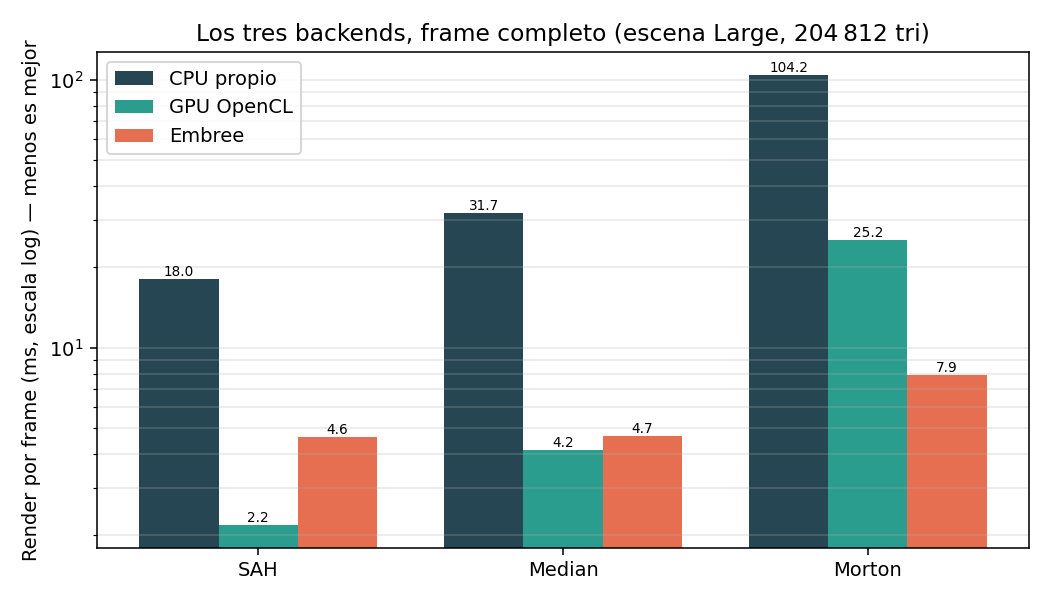
\includegraphics[width=\textwidth]{fig_backends.png}\\
\captionof{figure}{Los tres backends, frame completo (Large, escala log). CPU y
GPU usan \emph{nuestro} árbol y se disparan con Morton; Embree usa el suyo y
apenas cambia. Con buen árbol la GPU gana; con árbol malo, Embree es el más robusto.}
\end{minipage}\hfill
\begin{minipage}[t]{0.42\textwidth}\centering
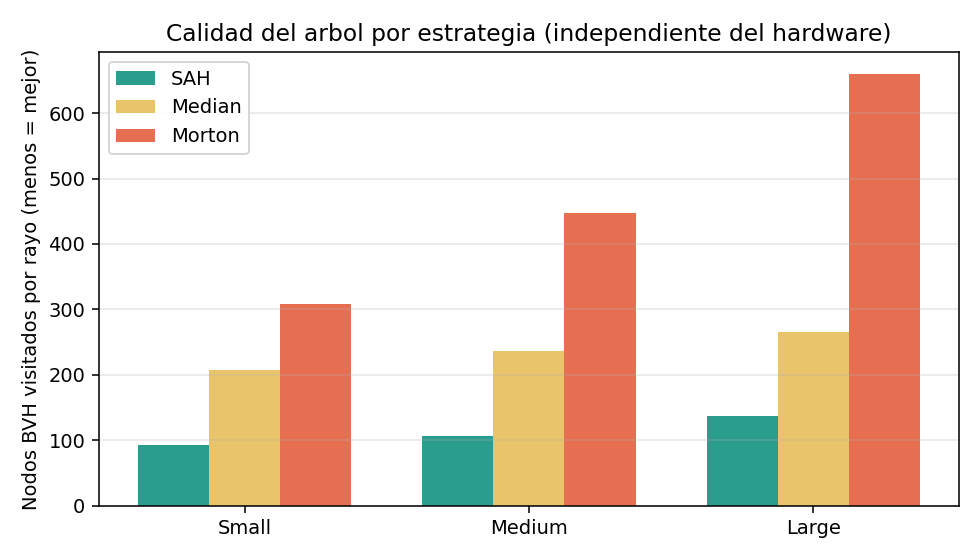
\includegraphics[width=\textwidth]{fig_quality.png}\\
\captionof{figure}{Calidad del árbol (nodos/rayo, menos es mejor): SAH domina en
toda densidad. La GPU hereda esta calidad al recorrer el mismo árbol.}
\end{minipage}
\end{figure}

\textbf{Análisis.} (i)~\emph{Heurística}: SAH visita $4.8\times$ menos nodos por
rayo que Morton ($138$ vs.\ $660$), lo que se traduce en un render en CPU
$\sim\!5.8\times$ más rápido; Morton solo gana en tiempo de \emph{build}. Como el
árbol estático se construye una vez y se recorre millones de veces, SAH es el
ganador global para geometría fija. (ii)~\emph{Hardware}: la GPU recorre el
\emph{mismo} árbol $4$--$10\times$ más rápido que la CPU; el paralelismo masivo
por píxel compensa el costo del \emph{flatten} y de la pila explícita, aun sin
hardware de trazado dedicado. (iii)~\emph{Ingeniería del recorrido}: el traversal
de Embree se mantiene en $\sim\!11$--$16$~ms aunque el árbol empeore de HIGH a
LOW, mientras que nuestro traversal escalar se dispara de $31$ a $116$~ms; la
brecha con Embree está en el \emph{kernel} SIMD/MBVH, no en la calidad del árbol.

\textbf{¿Y la geometría dinámica?} Repetimos el barrido reconstruyendo el árbol
\emph{cada frame} sobre una multitud escalable (Fig.~\ref{fig:dyn}). El
\emph{build} de Morton es el más barato, pero en esta escena sigue siendo pequeño
frente al traversal, así que SAH gana el costo por frame. La lectura no es que
``lo dinámico favorezca a SAH'', sino que \textbf{esta escena no es lo bastante
exigente} para que el \emph{build} domine: Morton solo convendría en un régimen
\emph{build-bound} (mucha más geometría, muchas reconstrucciones por frame, o muy
pocos rayos).

\begin{figure}[h]\centering
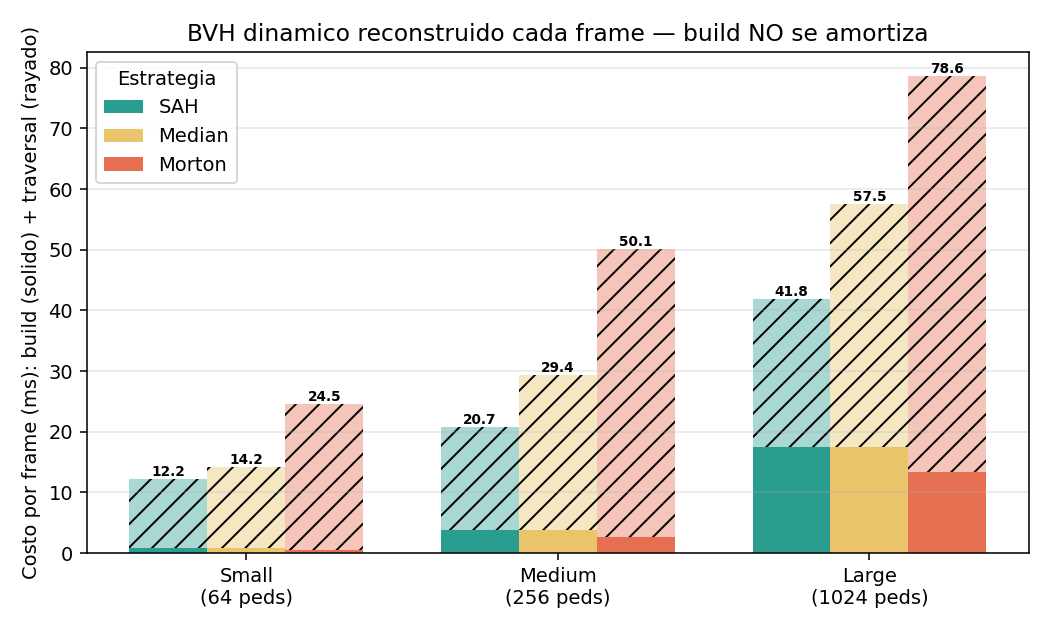
\includegraphics[width=0.44\textwidth]{fig_dynamic.png}
\caption{BVH reconstruido cada frame: costo $=$ \emph{build} (sólido) $+$
traversal (rayado). El \emph{build} de Morton es menor, pero su traversal lo
hunde y SAH gana el total igualmente.}
\label{fig:dyn}
\end{figure}
\section{Conclusiones}
Un \emph{benchmark} reproducible que, sobre la misma estructura y escena, separa
el efecto de la heurística del efecto del hardware. SAH ofrece el mejor árbol (y
el mejor render estático); la GPU acelera $4$--$10\times$ al portar el recorrido;
y la ventaja de Embree reside en la ingeniería SIMD de su recorrido, no en la
estructura ---una distinción central para un curso de estructuras de datos.
\textbf{Trabajo futuro}: recorrido SIMD y MBVH propios, construcción paralela,
\emph{refit} en vez de rebuild para lo dinámico, y comparación con SBVH.

\paragraph{Contribuciones por autor.} \emph{(a completar por el equipo)}
Kalos Lazo: BVH y heurísticas de construcción; Lenin Chávez: escena, sombreado y
renderer multihilo; Marcelo Chincha: backend OpenCL/GPU, integración de Embree y
\emph{benchmark}.

\paragraph{Enlaces.}
\begin{itemize}\setlength{\itemsep}{0pt}\setlength{\parskip}{0pt}\setlength{\topsep}{2pt}
  \item Repositorio: \url{https://github.com/marcelochincha/raytrec}
  \item Video demo: \href{https://drive.google.com/file/d/1uqEXMXC3iAAqOnv-YAQSjdeJ0dVSi4E4/view?usp=sharing}{Google Drive}
  \item Presentación: \href{https://drive.google.com/file/d/1Rf2MCSFvWEqkr26nSV0A_HS66tds9DNl/view?usp=sharing}{Google Drive}
\end{itemize}
\noindent{\small Datos y figuras en el repositorio: \texttt{docs/benchmark.csv},
\texttt{docs/fig\_*.png}, \texttt{docs/plot.py}.}

\begin{thebibliography}{9}\footnotesize\setlength{\itemsep}{0pt}
\bibitem{macdonald} J.~D. MacDonald y K.~S. Booth. \emph{Heuristics for ray
tracing using space subdivision}. The Visual Computer, 1990.
\bibitem{wald07} I.~Wald. \emph{On fast construction of SAH-based bounding volume
hierarchies}. IEEE Symp.\ on Interactive Ray Tracing, 2007.
\bibitem{lauterbach} C.~Lauterbach et al. \emph{Fast BVH construction on GPUs}.
Computer Graphics Forum (Eurographics), 2009.
\bibitem{karras} T.~Karras. \emph{Maximizing parallelism in the construction of
BVHs, octrees, and $k$-d trees}. High-Performance Graphics, 2012.
\bibitem{moller} T.~Möller y B.~Trumbore. \emph{Fast, minimum storage
ray/triangle intersection}. Journal of Graphics Tools, 1997.
\bibitem{embree} I.~Wald, S.~Woop, C.~Benthin, G.~S. Johnson y M.~Ernst.
\emph{Embree: a kernel framework for efficient CPU ray tracing}. ACM TOG
(SIGGRAPH), 2014.
\end{thebibliography}

\end{document}
